% !TeX root = surprises.tex

\chapter{Theorems From Geometry and Trigonometry}\label{a.trig}

%%%%%%%%%%%%%%%%%%%%%%%%%%%%%%%%%%%%%%%%%%%%%%%%%%%%%%%%%%%%%%%

In diesem Anhang werden Theoreme der Geometrie und Trigonometrie vorgestellt, die dem Leser möglicherweise nicht vertraut sind, sowie Theoreme, die zwar bekannt sind, deren Beweise jedoch nicht. Abschnitt~\ref{a.triangles} stellt drei Formeln zur Berechnung des Flächeninhalts eines Dreiecks vor. Abschnitt~\ref{a.trig-identities} beweist trigonometrische Identitäten. Obwohl die Formeln und Identitäten meist bekannt sind, lernen die Schüler diese Identitäten häufig auswendig oder schlagen sie nach, ohne jemals einen Beweis zu sehen. Die folgenden Abschnitte enthalten Beweise für fortgeschrittene Theoreme in der Geometrie: Abschnitt~\ref{a.bisector}---die Winkelhalbierungssätze, Abschnitt~\ref{a.ptolemy}---Ptolemäus' Theorem, das die Seiten und Diagonalen in einem Viereck, das von einem Kreis umschrieben wird, in Beziehung setzt, Abschnitt~\ref{a.ceva}---Cevas Lehrsatz über die drei Liniensegmente eines Dreiecks und Abschnitt~\ref{a.menelaus}---Menelaus' Lehrsatz über die Segmente einer Transversale in einem Dreieck.

%%%%%%%%%%%%%%%%%%%%%%%%%%%%%%%%%%%%%%%%%%%%%%%%%%%%%%%%%%%

\section{Theoreme über Dreiecke}\label{a.triangles}

%%%%%%%%%%%%%%%%%%%%%%%%%%%%%%%%%%%%%%%%%%%%%%%%%%%%%%%%%%%

\subsection{Berechnen des Flächeninhalts eines Dreiecks}


Die Standardformel zur Berechnung des Flächeninhalts eines Dreiecks aus der Basis und der Höhe ist bekannt. Sie kann mit verschiedenen geometrischen Methoden bewiesen werden.

\begin{theorem} Der Flächeninhalt des Dreiecks $\triangle ABC$ ist gegeben durch:
\begin{align}
\triangle ABC=\frac{1}{2}bh\,,\label{eq.area-from-base}
\end{align}
wobei $b$, die Basis, eine der Seiten des Dreiecks ist, und $h$, die Höhe, die Länge der Höhe zu $b$ vom gegenüberliegenden Scheitelpunkt (Abb.~\ref{f.area-base-height-1}).
\end{theorem}

\begin{proof}
Abbildung~\ref{f.area-base-height-2} zeigt, dass man die schraffierten Dreiecke so verschieben kann, dass sie ein Rechteck mit der gleichen Fläche wie das Dreieck bilden, wenn man das Dreieck in der Hälfte der Höhe "schneidet". Die Basis des Rechtecks ist $b$ und seine Höhe ist $h/2$.
\end{proof}

\begin{figure}[t]
\begin{minipage}{.45\textwidth}
\begin{tikzpicture}[scale=.7]
\coordinate (A) at (0,0);
\coordinate (C) at (7,0);
\path[name path=ab] (A) -- +(60:5.5);
\path[name path=cb] (C) -- +(140:7);
\path[name intersections={of=ab and cb,by={B}}];
\draw (A) -- node[below] {$b$} (C) -- node[above] {$a$} (B) -- node[above,xshift=-2pt] {$c$}  cycle;
\node[left] at (A) {$A$};
\node[above right,xshift=4pt] at (A) {$\theta$};
\node[above] at (B) {$B$};
\node[right] at (C) {$C$};
\draw (B) -- node[right,yshift=-4pt] {$h=c\sin\theta$} 
  (B|-A) coordinate (H);
\draw[rotate=90] (H) rectangle +(8pt,8pt);
\end{tikzpicture}
\caption{Berechnung des Flächeninhalts eines Dreiecks aus der Basis und der Höhe}\label{f.area-base-height-1}
\end{minipage}
\hfill
\begin{minipage}{.45\textwidth}
\begin{tikzpicture}[scale=.7]
\coordinate (A) at (0,0);
\coordinate (C) at (7,0);
\path[name path=ab] (A) -- +(60:5.5);
\path[name path=cb] (C) -- +(140:7);
\path[name intersections={of=ab and cb,by={B}}];
\node[left] at (A) {$A$};
\node[above] at (B) {$B$};
\node[right] at (C) {$C$};
\path (B) -- node[right,near end] {$h/2$} (B|-A) coordinate (H);
\draw[rotate=90] (H) rectangle +(8pt,8pt);
\coordinate (K) at ($(H)!.5!(B)$);
\draw (A) -- node[below] {$b$} (C);
\draw (H) -- (K);
\coordinate (KA) at (K -| A);
\coordinate (KAB) at ($(A)!.5!(B)$);
\fill[color=white!50!red] (A) -- (KA) -- (KAB) -- cycle;
\fill[color=white!50!red] (B) -- (KAB) -- (K) -- cycle;
\coordinate (KC) at (K -| C);
\coordinate (KBC) at ($(B)!.5!(C)$);
\fill[color=white!50!blue] (C) -- (KC) -- (KBC) -- cycle;
\fill[color=white!50!blue] (B) -- (KBC) -- (K) -- cycle;
\draw[very thick,dashed] (A) -- (K -| A) -- (K -| C) -- (C);
\draw[very thick,dashed] (A) -- (B) -- (K);
\draw[very thick,dashed] (B) -- (C);
\path (K) -- node[inner sep=1pt, fill=white,right,
                 xshift=2pt,yshift=-3pt] {$h/2$} (B);
\end{tikzpicture}
\caption{Berechnung des Flächeninhalts eines Dreiecks aus der Basis und der Höhe}\label{f.area-base-height-2}
\end{minipage}
\end{figure}

\begin{theorem} Der Flächeninhalt des Dreiecks $\triangle ABC$ ist gegeben durch:
\begin{align}\label{eq.area-from-sine}
\triangle ABC = \frac{1}{2}bc\sin \theta\,.
\end{align}
\end{theorem}
\begin{proof} Aus Thm.~\ref{eq.area-from-base} mit
$h=c\sin \theta$.
\end{proof}

%%%%%%%%%%%%%%%%%%%%%%%%%%%%%%%%%%%%%%%%%%%%%%%%%%%%%%%%%%%


\begin{theorem}[Heron] Der Flächeninhalt des Dreiecks $\triangle ABC$ ist gegeben durch:\label{thm.heron} 
\[
\triangle ABC = \sqrt{s(s-a)(s-b)(s-c)}\,,
\]
wobei $s$, der Halbkreisumfang des Dreiecks, gleich ist $\frac{1}{2}(a+b+c)$.
\end{theorem}

\begin{proof}
Ein Radius eines Kreises und eine Tangente, die den Radius schneidet, stehen senkrecht zueinander. Außerdem sind die Längen der Linienabschnitte zweier Tangenten vom gleichen Punkt zum Kreis gleich. Dies zeigt, dass der Mittelpunkt des Dreiecks, der Mittelpunkt des Inkreises, der gemeinsame Schnittpunkt der drei Winkelhalbierenden ist.
\[
\triangle AOB'\cong \triangle AOC',\quad
\triangle BOA'\cong\triangle BOC',\quad
\triangle COA'\cong \triangle COB'\,.
\]
\begin{figure}[ht]
\begin{center}
\begin{tikzpicture}[scale=1.8]
% Draw base and path two lines at known angles
\draw (0,0) coordinate (a) node[xshift=-6pt] {$A$} -- (0:6) coordinate (b) node[xshift=6pt] {$B$};
\path[name path=ac] (a) -- +(50:4);
\path[name path=bc] (b) -- +(150:5);
% Get their intersection and draw lines between vertices
\path[name intersections={of=ac and bc,by=c}];
\node[above] at (c) {$C$};
\draw (a) -- (c) -- (b) -- (a);
% Label angles with tick marks
\draw (a) ++(0:4mm) arc (0:50:4mm);
\draw (a) ++(10:3.5mm) -- +(10:1mm);
\draw (a) ++(15:3.5mm) -- +(15:1mm);
\draw (a) ++(35:3.5mm) -- +(35:1mm);
\draw (a) ++(40:3.5mm) -- +(45:1mm);
\draw (b) ++(150:5mm) arc (150:180:5mm);
\draw (b) ++(157.5:4.5mm) -- +(157.5:1mm);
\draw (b) ++(172.5:4.5mm) -- +(172.5:1mm);
\draw (c) ++(230:3mm) arc (230:330:3mm);
\draw (c) ++(250:2.4mm) -- +(250:.9mm);
\draw (c) ++(255:2.4mm) -- +(255:.9mm);
\draw (c) ++(260:2.4mm) -- +(260:.9mm);
\draw (c) ++(300:2.4mm) -- +(300:.9mm);
\draw (c) ++(305:2.4mm) -- +(305:.9mm);
\draw (c) ++(310:2.4mm) -- +(310:.9mm);
% Path bisectors of two lines
\path[name path=bia] (a) -- +(25:3.5);
\path[name path=bib] (b) -- +(165:5);
% Intersection of angle bisectors
\path [name intersections={of=bia and bib,by=center}];
% Draw angle bisectors to center
\draw (a) -- (center);
\draw (c) -- (center);
\draw (b) -- (center);
% Draw radii
\draw (center) -- node[left] {$r$} ($(a)!(center)!(b)$) node[below,yshift=-2pt] {$C'$} coordinate (ap);
\draw (center) -- node[left,yshift=-4pt] {$r$} ($(a)!(center)!(c)$) node[above left] {$B'$} coordinate (bp);
\draw (center) -- node[right] {$r$} ($(b)!(center)!(c)$) node[above right] {$A'$} coordinate (cp);
% Draw dots
\vertex{center};
\node[above,xshift=3pt,yshift=7pt] at (center) {$O$};
% Draw right angle squares
\draw (ap) -- ++(90:4pt) -- ++(0:4pt) -- ++(-90:4pt);
\draw (bp) -- ++(-40:4pt) -- ++(-130:4pt) -- ++(-220:4pt);
\draw (cp) -- ++(-30:4pt) -- ++(-120:4pt) -- ++(-210:4pt);
% Labels of angles
\node[above,xshift=5pt,yshift=18pt] at (center) {$\gamma/2$};
\node[above left,xshift=-4pt,yshift=18pt] at (center) {$\gamma/2$};
\node[above right,xshift=3pt,yshift=-3pt] at (center) {$\beta/2$};
\node[below right,yshift=-3pt] at (center) {$\beta/2$};
\node[left,xshift=-5pt,yshift=2pt] at (center) {$\alpha/2$};
\node[below left,xshift=2pt,yshift=-4pt] at (center) {$\alpha/2$};
% Labels of line segments (names of points are weird...)
\path (a) -- node[below,yshift=-2pt] {$u$} (ap);
\path (a) -- node[left, xshift=-2pt] {$u$} (bp);
\path (b) -- node[above,yshift=2pt]  {$v$} (cp);
\path (b) -- node[below,xshift=-2pt] {$v$} (ap);
\path (c) -- node[above,xshift=-2pt] {$w$} (bp);
\path (c) -- node[above,xshift=2pt]  {$w$} (cp);
% Labels of sides
\draw[<->] ($(a)+(0,-10pt)$) -- node[fill=white] {$c$} 
           ($(b)+(0,-10pt)$);
\draw[<->] ($(a)+(-10pt,8pt)$) -- node[fill=white] {$b$}
           ($(c)+(-10pt,8pt)$);
\draw[<->] ($(b)+(6pt,10pt)$) -- node[fill=white] {$c$}
           ($(c)+(6pt,10pt)$);
% Inscribed circle
\node[very thick,dotted,draw,circle through=(ap)] at (center) {};
\end{tikzpicture}
\end{center}
\caption{Dreieck mit eingeschriebenem Kreis}\label{f.inscribed}
\end{figure}
Die Fläche $\triangle ABC$ ist die Summe der sechs oben aufgeführten Dreiecke. Da die Höhe von sechs Dreiecken $r$, dem Radius des Inkreises, entspricht, erhalten wir:
\begin{subeqnarray}
\triangle ABC&=&\triangle AOB'\!+\!\triangle AOC'\!+\!\triangle BOA'\!+\!\triangle BOC'\!+\!\triangle COA'\!+\!\triangle COB'\\
\triangle ABC&=&\frac{1}{2}r(u+u+v+v+w+w)\\
\triangle ABC&=&\frac{1}{2}r(a+b+c)\\
\triangle ABC&=&rs \slabel{eq.area-heron}\,.
\end{subeqnarray}
Definieren wir nun die Seiten in Bezug auf die Tangenten der zentralen Winkel:
\begin{displaymath}
\tan \frac{\alpha}{2} = \frac{u}{r},\quad
\tan \frac{\beta}{2} = \frac{v}{r},\quad
\tan \frac{\gamma}{2} = \frac{w}{r}\,.
\end{displaymath}
Aus diesen Definitionen und $s=\frac{1}{2}(2u+2u+2w)$ erhalten wir:
\[
s = u+v+w = r\left(\tan \frac{\alpha}{2}+\tan \frac{\beta}{2}+\tan \frac{\gamma}{2}\right)\,.
\]
Seit $\frac{\alpha}{2}+\frac{\alpha}{2}+\frac{\beta}{2}+\frac{\beta}{2}+\frac{\gamma}{2}+\frac{\gamma}{2}=360^\circ$ und somit $\frac{\alpha}{2}+\frac{\beta}{2}+\frac{\gamma}{2}=180^\circ$, von Thm.~\ref{thm.tangent3}:
\begin{eqnarray*}
s&=&r\left(\tan \frac{\alpha}{2}\tan \frac{\beta}{2}\tan \frac{\gamma}{2}\right)\\
&=&r\left(\frac{u}{r}\frac{v}{r}\frac{w}{r}\right)=\frac{1}{r^2}(u\,v\,w)\\
r&=&\sqrt{\displaystyle\frac{u\,v\,w}{s}}\,.
\end{eqnarray*}
Von Eq.~\ref{eq.area-heron}:
\[
\triangle ABC=rs=s\sqrt{\displaystyle\frac{u\,v\,w}{s}}=\sqrt{s\,u\,v\,w}\,.
\]
Die Heronsche Formel ergibt sich aus $u=s-a, v=s-b, w=s-c$.
\end{proof}


%%%%%%%%%%%%%%%%%%%%%%%%%%%%%%%%%%%%%%%%%%%

\section{Trigonometrische Identitäten}\label{a.trig-identities}



%%%%%%%%%%%%%%%%%%%%%%%%%%%%%%%%%%%%%%%%%%%%%%%%%%%%%%%%%%%

\subsection{Sinus und Kosinus der Summe und Differenz zweier Winkel} \label{s.sum-of-trig}

\begin{theorem}\label{thm.sum-of-trig}
\begin{eqnarray*}
\sin(\alpha+\beta) &=& \sin\alpha\cos\beta + \cos\alpha\sin\beta\\
\sin(\alpha-\beta) &=& \sin\alpha\cos\beta - \cos\alpha\sin\beta\\
\cos(\alpha+\beta) &=& \cos\alpha\cos\beta - \sin\alpha\sin\beta\\
\cos(\alpha-\beta) &=& \cos\alpha\cos\beta + \sin\alpha\sin\beta\,.
\end{eqnarray*}
\end{theorem}
Wir werden die erste Formel beweisen; die anderen Formeln können mit Hilfe der Werte von Sinus und Kosinus für $-\alpha$ und $90^\circ-\alpha$ erhalten werden.

Ausgehend von einem rechtwinkligen Dreieck $\triangle ABC$ mit spitzem Winkel $\alpha$ und einem rechtwinkligen Dreieck $\triangle ACD$ mit spitzem Winkel $\beta$ können wir sie zu geometrischen Figuren mit einem Winkel $\alpha+\beta$ verbinden (Abb.~\ref{f.sin-sum1}). Das linke Diagramm wird am häufigsten in den Beweisen der Identitäten verwendet. Hier geben wir zwei Beweise, die auf dem mittleren und dem rechten Diagramm basieren.
\begin{figure}[ht]
\begin{center}
\begin{tikzpicture}[scale=.85]
\coordinate (A) at (0,0);
\node[below] at (A) {$A$};
\node[right,xshift=6pt,yshift=4pt] at (A) {$\alpha$};
\node[above right,xshift=6pt,yshift=8pt] at (A) {$\beta$};
\coordinate (B) at (3,0);
\node[below] at (B) {$B$};
\path[name path=ac1] (A) -- +(40:4.5);
\path[name path=bc1] (B) -- +(90:3.5);
\path[name intersections={of=ac1 and bc1,by={C}}];
\node[above right] at (C) {$C$};
\draw (A) -- (B) -- (C) -- cycle;
\draw (C) -- ($(C)!2cm!-90:(A)$) coordinate (D) -- (A);
\node[above] at (D) {$D$};
\draw[rotate=90] (B) rectangle +(7pt,7pt);
\draw[rotate=128] (C) rectangle +(7pt,7pt);

\begin{scope}[xshift=4.3cm]
\coordinate (B) at (0,0);
\node[below] at (B) {$B$};
\coordinate (D) at (4,0);
\node[below] at (D) {$D$};
\draw (B) -- +(70:4) coordinate (A);
\node[above] at (A) {$A$};
\draw (A) -- (B) -- (D) -- cycle;

\draw (A) -- (A|-B) coordinate (C);
\node[below] at (C) {$C$};
\node[below left,xshift=2pt,yshift=-18pt] at (A) {$\alpha$};
\node[below right,xshift=0pt,yshift=-14pt] at (A) {$\beta$};
\draw[rotate=90] (C) rectangle +(7pt,7pt);
\draw (C) rectangle +(7pt,7pt);
\end{scope}

\begin{scope}[xshift=9.75cm]
\coordinate (A) at (0,0);
\node[below] at (A) {$A$};
\node[right,xshift=6pt,yshift=5pt] at (A) {$\alpha$};
\node[above right,xshift=4pt,yshift=8pt] at (A) {$\beta$};
\coordinate (B) at (3.5,0);
\node[below] at (B) {$B$};
\draw (A) -- +(70:4.5) coordinate (D);
\node[above] at (D) {$D$};
\path[name path=dc1] (D) -- +(-20:2.5);
\path[name path=bc1] (B) -- +(90:4);
\path[name intersections={of=dc1 and bc1,by={C}}];
\node[above] at (C) {$C$};
\draw[rotate=90] (B) rectangle +(7pt,7pt);
\draw[rotate=-110] (D) rectangle +(7pt,7pt);
\draw (A) -- (B) -- (C) -- (D) -- cycle;
\draw (A) -- (C);
\end{scope}
\end{tikzpicture}
\end{center}
\caption{Diagramme zum Nachweis der Identität für den Sinus von Winkelsummen}\label{f.sin-sum1}
\end{figure}

\begin{proof}
(1)
Berechnen wir den Flächeninhalt von $\triangle ABD$ auf zwei verschiedene Arten: (1) mit Hilfe von Gl.~\ref{eq.area-from-sine} für $\triangle ABD$, und (2) mit Hilfe der Gleichung getrennt für $\triangle ABC$ und $\triangle ADC$ (Fig.~\ref{f.sin-sum2}).
Auch $h$ wird zweimal mit Hilfe der Definition der trigonometrischen Funktionen berechnet:
\begin{eqnarray*}
\triangle ABD &=& \frac{1}{2}bc\sin(\alpha+\beta)\\
\triangle ABD &=& \triangle ABC+\triangle ADC\\
&=& \frac{1}{2}ch\sin \alpha + \frac{1}{2}bh\sin \beta\\
&=& \frac{1}{2}c(b\cos\beta)\sin \alpha + \frac{1}{2}b(c\cos\alpha)\sin \beta\,.
\end{eqnarray*}
Wenn man die beiden Formeln für $\triangle ABD$ gleichsetzt und $\frac{1}{2}bc$ aufhebt, erhält man:
\[
\sin(\alpha+\beta)=\sin\alpha\cos\beta+\cos \alpha\sin\beta\,.
\]
\end{proof}

\begin{figure}[tb]
\begin{center}
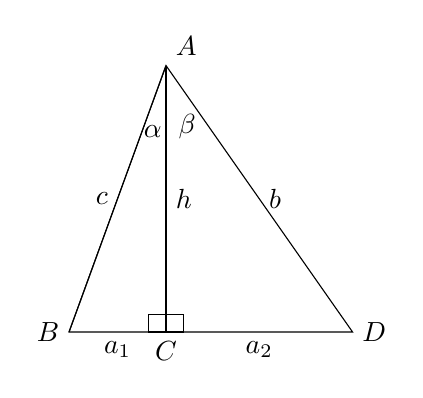
\begin{tikzpicture}[scale=.9]
\coordinate (B) at (0,0);
\node[left] at (B) {$B$};
\coordinate (D) at (4,0);
\node[right] at (D) {$D$};
\draw (B) -- +(70:4) coordinate (A);
\node[above right] at (A) {$A$};
\draw (A) -- node[left] {$c$} (B) -- (D) -- node[right] {$b$} cycle;

\draw (A) -- node[right] {$h$} (A|-B) coordinate (C);
\node[below] at (C) {$C$};
\node[below left,xshift=2pt,yshift=-18pt] at (A) {$\alpha$};
\node[below right,xshift=1pt,yshift=-14pt] at (A) {$\beta$};
\draw[rotate=90] (C) rectangle +(7pt,7pt);
\draw (C) rectangle +(7pt,7pt);
\path (B) -- node[below] {$a_1$} (C) -- node[below] {$a_2$} (D);
\end{tikzpicture}
\end{center}
\caption{Berechnung des Flächeninhalts eines Dreiecks auf zwei Arten}\label{f.sin-sum2}
\end{figure}

Der zweite Beweis beruht auf folgendem Satz:
\begin{theorem}
In einem Kreis mit einem Durchmesser von $1$ ist die Länge einer Sehne, die einen eingeschriebenen Winkel einschließt, gleich dem Sinus des Winkels (Abb.~\ref{f.chord-angle}).
\end{theorem}

\begin{figure}[b]
\begin{center}
\begin{tikzpicture}[scale=.7]
\coordinate (A) at (0,0);
\coordinate (C) at (3,4);
\coordinate (O) at ($(A)!.5!(C)$);
\vertex{O};
\node[left] at (O) {$O$};
\draw (A) -- (C);
\node[draw,circle through=(A),name path=circle] at (O) {};
\coordinate (B) at ($(O)+(10:2.5)$);
\draw (A) -- (B) -- node[left] {$a$} (C);
\draw[rotate=120] (B) rectangle +(8pt,8pt);
\coordinate (D) at ($(O)+(160:2.5)$);
\draw(C) -- (D) -- (B);
\node[above right,xshift=12pt,yshift=12pt] at (A) {$\alpha$};
\node[right,xshift=16pt,yshift=2pt] at (D) {$\alpha$};
\node[below left] at (A) {$A$};
\node[above right] at (C) {$B$};
\node[right] at (B) {$C$};
\node[left] at (D) {$D$};
\end{tikzpicture}
\end{center}
\caption{Alle von einer Sehne eingeschlossenen Winkel sind gleich}\label{f.chord-angle}
\end{figure}

\begin{proof}
Sei $\overline{AB}$ ein Durchmesser und sei $\angle BAC=\alpha$. Sei $D$ ein beliebiger anderer Punkt auf dem Kreis, der ein Dreieck $\triangle BDC$ bildet, dessen eine Seite die Sehne $\overline{BC}$ ist. Da gleiche Sehnen gleiche Inkreiswinkel einschließen, sei $\angle BDC=\alpha$. Im rechtwinkligen Dreieck $\triangle ABC$:
\[
\sin \alpha = \frac{\overline{BC}}{\overline{AB}}=\frac{\overline{BC}}{1}=\overline{BC}\,.
\]
\end{proof}

\begin{proof}(2)
Dieser Beweis basiert auf dem rechten Diagramm in Abb.~\ref{f.sin-sum1}, das in Abb.~\ref{f.trig-quad-circle} wiedergegeben ist, wo das Viereck $\overline{ABCD}$ in einen Kreis eingeschrieben wurde.
Nach Thm.~\ref{thm.quad-circum} kann ein Viereck dann und nur dann von einem Kreis umschrieben werden, wenn die Summe jedes Paares gegenüberliegender Winkel $180^\circ$ ist.
$\angle ADC+\angle ABC=180^\circ$, da beide Winkel rechtwinklig sind. Aus Thm.~\ref{thm.interior-angles-of-a-polygon} ist die Summe der Innenwinkel eines Vierecks $360^\circ$, also $\angle DAB+\angle DCB=180^\circ$. 
\begin{figure}[t]
\begin{center}
\begin{tikzpicture}[scale=.8]
\coordinate (A) at (0,0);
\node[left] at (A) {$A$};
\node[right,xshift=6pt,yshift=5pt] at (A) {$\alpha$};
\node[above right,xshift=4pt,yshift=8pt] at (A) {$\beta$};
\coordinate (B) at (3.5,0);
\node[right] at (B) {$B$};
\draw (A) -- +(70:4.5) coordinate (D);
\node[above left] at (D) {$D$};
\path[name path=dc1] (D) -- +(-20:2.5);
\path[name path=bc1] (B) -- +(90:4);
\path[name intersections={of=dc1 and bc1,by={C}}];
\node[above right] at (C) {$C$};
\draw[rotate=90] (B) rectangle +(9pt,9pt);
\draw[rotate=-110] (D) rectangle +(9pt,9pt);
\draw (A) -- (B) -- (C) -- (D) -- cycle;
\draw (A) -- (C);
\draw (D) -- (B);

\coordinate (O) at ($(A)!.5!(C)$);
\node[draw,circle through=(A),name path=circle] at (O) {};
\node[below right,xshift=6pt,yshift=-4pt] at (D) {$\alpha$};
\node[below,xshift=1pt,yshift=-10pt] at (D) {$\gamma$};
\node[below left,xshift=-6pt,yshift=4pt] at (C) {$\delta$};
\node[below,xshift=-4pt,yshift=-6pt] at (C) {$\gamma$};
\node[above left,xshift=-7pt,yshift=4pt] at (B) {$\delta$};
\node[above,xshift=-4pt,yshift=14pt] at (B) {$\beta$};
\end{tikzpicture}
\end{center}
\caption{Ein Viereck, das von einem Kreis umschrieben wird}\label{f.trig-quad-circle}
\end{figure}
Der Durchmesser des Kreises sei $1$ (ansonsten alles mit der Länge des Durchmessers multiplizieren). Dann sind die Seiten des Vierecks:
\[
\overline{BC}=\sin\alpha,\quad \overline{CD}=\sin\beta,\quad \overline{AB}=\sin\gamma,\quad \overline{DA}=\sin\delta\,,
\]
und ihre Diagonalen sind:
\[
\overline{BD}=\sin(\alpha + \beta),\quad \overline{CA}=\sin (\alpha+\gamma)\,.
\]
Nach dem Satz des Ptolemäus (Thm.~\ref{thm.ptolemy}) ist das Produkt der Diagonalen eines Vierecks, das von einem Kreis umschrieben wird, gleich der Summe der Produkte der gegenüberliegenden Seiten des Vierecks. Da $\angle ADC$ und $\angle ABC$ rechte Winkel sind, haben wir:
\[
\renewcommand{\arraystretch}{1.3}
\begin{array}{lcl}
\sin (\alpha+\beta)\sin(\alpha+\gamma)&=&
\sin \alpha \sin\delta + \sin \beta\sin \gamma\\
\sin (\alpha+\beta)\sin(90^\circ)&=&
\sin \alpha \sin(90^\circ-\beta) + \sin \beta\sin (90^\circ-\alpha)\\
\sin (\alpha+\beta)&=&\sin\alpha\cos\beta+\cos\alpha\sin \beta\,.
\end{array}
\]
\end{proof}

%%%%%%%%%%%%%%%%%%%%%%%%%%%%%%%%%%%%%%%%%%%%%%%%%%%%%%%%%%%

\subsection{Der Kosinus eines Dreifachwinkels}\label{s.cosine}

\begin{theorem}\label{thm.triple-angle}
\[
\cos 3\alpha=4\cos^3\alpha -3\cos\alpha\,.
\]
\end{theorem}
\begin{proof}
Der Beweis verwendet die Formeln in Thm.~\ref{thm.sum-of-trig} und die Formel $\sin^2\alpha+\cos^2\alpha=1$:
\begin{eqnarray*}
\cos 3\alpha &=& \cos (2\alpha +\alpha)\\
&=& \cos 2\alpha\cos\alpha - \sin 2\alpha\sin\alpha\\
&=& (\cos^2\alpha -\sin^2\alpha)\cos\alpha - (2\sin\alpha\cos\alpha)\sin\alpha\\
&=&\cos^3\alpha - \cos\alpha\sin^2\alpha -2\sin^2\alpha\cos\alpha)\\
&=&\cos^3\alpha - \cos\alpha +\cos^3\alpha -2\cos\alpha+2\cos^3\alpha\\
&=&4\cos^3\alpha -3\cos\alpha\,.
\end{eqnarray*}
\end{proof}

%%%%%%%%%%%%%%%%%%%%%%%%%%%%%%%%%%%%%%%%%%%%%%%%%%%%%%%%%%%

\subsection{Sinus und Kosinus eines Halbwinkels}\label{s.sine-cosine-half}

\begin{theorem}\label{thm.sine-cosine-half}
Wenn $\alpha$ ein Winkel in einem \emph{Dreieck} ist, dann:\footnote{Die allgemeine Formel ist komplexer, weil die Quadratwurzeln entweder positiv oder negativ sein können, je nachdem, in welchem Quadranten $\alpha/2$ liegt. Für ein Dreieck $0\!<\!\alpha\!<\!180^\circ$ liegt also $0\!<\!\alpha/2\!<\!90^\circ$ im ersten Quadranten und sowohl der Sinus als auch der Kosinus sind positiv.}
\begin{eqnarray*}
\cos \left(\frac{\alpha}{2}\right)&=&\sqrt{\frac{1+\cos\alpha}{2}}\\
\sin\left(\frac{\alpha}{2}\right)&=&\sqrt{\frac{1-\cos\alpha}{2}}\,.
\end{eqnarray*}
\end{theorem}

\begin{proof}
Der Beweis verwendet die Formeln Thm.~\ref{thm.sum-of-trig} und die Formel $\sin^2\alpha+\cos^2\alpha=1$:
\begin{eqnarray*}
\cos \alpha&=&\cos 2\left(\frac{\alpha}{2}\right)=\cos \left(\frac{\alpha}{2}\right)\cos\left(\frac{\alpha}{2}\right)-\sin \left(\frac{\alpha}{2}\right)\sin\left(\frac{\alpha}{2}\right)\\
&=&2\cos^2 \left(\frac{\alpha}{2}\right)-1\\
\cos \left(\frac{\alpha}{2}\right)&=&\sqrt{\frac{1+\cos\alpha}{2}}\\
\sin^2\left(\frac{\alpha}{2}\right)&=& 1-\cos^2\left(\frac{\alpha}{2}\right)=1-\frac{1+\cos\alpha}{2}\\
\sin \left(\frac{\alpha}{2}\right)&=&\sqrt{\frac{1-\cos\alpha}{2}}\,.
\end{eqnarray*}
\end{proof}

%%%%%%%%%%%%%%%%%%%%%%%%%%%%%%%%%%%%%%%%%%%%%%%%%%%%%%%%%%%

\subsection{Das Kosinusgesetz}

\begin{theorem}[Law of cosines]
In einem Dreieck $\triangle ABC$ mit den Seiten $a,b,c$ (Abb.~\ref{f.law-cosines2}):\label{thm.law-of-cosines}
\[
c^2=a^2+b^2-2ab\cos \angle ACB\,.
\]
\end{theorem}

\begin{proof}(1)
Ziehe eine Höhe von $C$ nach $\overline{AB}$ und verwende die Definition des Kosinus und den Satz des Pythagoras:
\begin{subeqnarray}
c&=& x+(c-x)=a\cos \beta + b\cos \alpha\\
c^2&=&ac\cos \beta + bc\cos \alpha\,.\slabel{eq.lc1}
\end{subeqnarray}
In ähnlicher Weise fallen die Höhen von $A$ bis $\overline{BC}$ und von $B$ bis $\overline{AC}$, um zu erhalten:
\begin{subeqnarray}
a^2&=&ca\cos \beta + ba\cos \gamma\slabel{eq.lc2}\\
b^2&=&cb\cos \alpha + ab\cos \gamma\,.\slabel{eq.lc3}
\end{subeqnarray}
Die Addition der Gleichungen ~\ref{eq.lc2} und \ref{eq.lc3} und die Subtraktion der Gleichung ~\ref{eq.lc1} ergibt:
\begin{eqnarray*}
a^2+b^2-c^2&=&ca\cos \beta + ba\cos \gamma\\
&&\;\; +\,cb\cos \alpha + ab\cos \gamma \\
&&\;\; -\,ac\cos \beta - bc\cos \alpha\\
&=&2ab\cos \gamma\\
c^2&=&a^2+b^2-2ab\cos \gamma\,.
\end{eqnarray*}
\end{proof}

\begin{figure}[b]
\begin{center}
\begin{tikzpicture}[scale=.65]
  \coordinate[label = left:$A$] (A) at (0,0);
  \coordinate[label = right:$B$] (B) at (6,0);
  \draw (A) -- (40:5) coordinate (C) node[above] {$C$};
  \draw (A) -- (B) -- node[right] {$a$} (C) -- node[left,yshift=4pt,xshift=-2pt] {$b$} cycle;
\node[below,xshift=-4pt,yshift=-6pt] at (C) {$\gamma$};
\node[above right,xshift=8pt] at (A) {$\alpha$};
\node[above left,xshift=-8pt] at (B) {$\beta$};
\coordinate (D) at (A-|C);
\draw (C) -- (D);  
\draw (D) rectangle +(10pt,10pt);
\draw[<->] (0,-.5) -- node[fill=white] {$c$} (6,-0.5);
\draw[<->] (0,-1) -- node[fill=white] {$c-x$} ($(D)+(0,-1)$);
\draw[<->] ($(D)+(0,-1)$) -- node[fill=white] {$x$} (6,-1);
\end{tikzpicture}
\caption{Beweis 1 für das Kosinusgesetz}\label{f.law-cosines2}
\end{center}
\end{figure}

\begin{proof}(2)
Der zweite Beweis verwendet den Satz des Ptolemäus (Thm.~\ref{thm.ptolemy}).\footnote{Abschnitt~\ref{a.ptolemy} verwendet das Kosinussatzgesetz zum Beweis des Satzes des Ptolemäus! Der erste Beweis des Kosinussatzes vermeidet diesen Zirkelschluss. Außerdem gibt es Beweise für den Satz des Ptolemäus, die das Kosinussatzgesetz nicht verwenden.}

Das Dreieck $\triangle ABC$ kann von einem Kreis umschrieben werden. 
Konstruieren Sie ein weiteres Dreieck $\triangle ABC'$, das kongruent zu $\triangle ABC$ ist und in denselben Kreis eingeschrieben ist (Abb.~\ref{f.law-cosines3}). Dazu konstruiert man einen Winkel von $\overline{AB}$ gleich $\angle CAB$, der den Kreis in $C'$ schneidet, und konstruiert dann die Linie $\overline{C'A}$.
Da Winkel, die durch dieselbe Sehne aufgespannt werden, gleich sind $\angle AC'B =\angle BCA$, so ist auch $\angle CBA=\angle C'AB$ und damit $\triangle ABC'\cong\triangle BAC$ durch Winkel-Seiten-Winkel mit der gemeinsamen Seite $\overline{AB}$.

Fallen Sie die Lote von $C$ nach $D$ und von $C'$ nach $D'$ auf $\overline{AB}$, so dass $x=a\cos \beta$. Nach dem Satz des Ptolemäus für das Viereck $\overline{ABCC'}$:
\begin{eqnarray*}
b^2&=&a^2+c(c-2x)\\
&=& a^2 + c(c-2a\cos\beta)\\
&=&a^2+c^2-2ac\cos\beta\,.
\end{eqnarray*}
\end{proof}

\begin{figure}[b]
\begin{center}
\begin{tikzpicture}[scale=.8]
\coordinate (origin) at (0,0);
\coordinate (A) at (-3,-1.5);
\coordinate (B) at (3,-1.5);
\node[draw,circle through=(A),name path=circle] at (origin) {};
\node[left] at (A) {$A$};
\node[right] at (B) {$B$};
\path[name path=b1] (A) -- +(40:7cm);
\path[name path=b2] (B) -- +(140:7cm);
\path [name intersections={of=circle and b1,by={C}}];
\node[above] at (C) {$C$};
\path [name intersections={of=circle and b2,by={Cp}}];
\node[above] at (Cp) {$C'$};
\draw (A) -- node[below] {$c$} (B) -- node[right] {$a$} (C) -- node[left,yshift=4pt,xshift=-2pt] {$b$} cycle;
\draw (A) -- (B) -- node[right,yshift=4pt,xshift=2pt] {$b$}(Cp) -- node[left] {$a$} cycle;
\draw (C) -- node[above] {$c-2x$} (Cp);
\coordinate (D) at (C|-B);
\coordinate (Dp) at (Cp|-B);
\draw (C) -- (D);
\draw[rotate=90] (D) rectangle +(8pt,8pt);
\draw (Cp) -- (Dp);
\draw (Dp) rectangle +(8pt,8pt);
\draw[<->] ($(A)+(0,-.8)$) -- node[fill=white] {$x$} ($(Dp)+(0,-.8)$);
\draw[<->] ($(Dp)+(0,-.8)$) -- node[fill=white] {$c-2x$} ($(D)+(0,-.8)$);
\draw[<->] ($(D)+(0,-.8)$) -- node[fill=white] {$x$} ($(B)+(0,-.8)$);
\node[below] at (D) {$D$};
\node[below] at (Dp) {$D'$};
\node[above right,xshift=8pt,yshift=6pt] at (B) {$\beta$};
\draw ($(B)+(-.8,0)$) arc (180:104:.8);
\draw[->] ($(B)+(.4,.5)$) -- +(190:1.12);

\node[above left,xshift=-8pt,yshift=6pt] at (A) {$\beta$};
\draw ($(A)+(.8,0)$) arc (0:76:.8);
\draw[->] ($(A)+(-.4,.5)$) -- +(-10:1.12);
\end{tikzpicture}
\end{center}
\caption{Beweis 2 für das Kosinusgesetz}\label{f.law-cosines3}
\end{figure}                       

%%%%%%%%%%%%%%%%%%%%%%%%%%%%%%%%%%%%%%%%%%%%%%%%%%%%%%%%%%%

\subsection{Der Tangens der Summe von zwei Winkeln}\label{s.tangent-sum}


\begin{theorem}\label{thm.tangent-sum}
\[
\tan (\alpha+\beta) =\frac{\tan\alpha+\tan\beta}{1-\tan\alpha\tan\beta}\,.
\]
\end{theorem}

\begin{proof}
\begin{eqnarray*}
\tan (\alpha+\beta) &=& \frac{\sin(\alpha+\beta)}{\cos(\alpha+\beta)}\\
&=&\frac{\sin\alpha\cos\beta+\cos\alpha\sin\beta}{\cos\alpha\cos\beta-\sin\alpha\sin\beta}\\
&=&\frac{\sin\alpha+\cos\alpha\tan\beta}{\cos\alpha-\sin\alpha\tan\beta}\\
&=&\frac{\tan\alpha+\tan\beta}{1-\tan\alpha\tan\beta}\,.
\end{eqnarray*}
\end{proof}

%%%%%%%%%%%%%%%%%%%%%%%%%%%%%%%%%%%%%%%%%%%%%%%%%%%%%%%%%%%

\subsection{Der Tangens eines Halbwinkels}\label{s.tangent-half}

\begin{theorem}\label{thm.tangent-half}
\[
\tan\left(\frac{\alpha}{2}\right) = \frac{-1\pm\sqrt{1+\tan^2\alpha}}{\tan\alpha}\,.
\]
\end{theorem}
\begin{proof}
Wir leiten eine quadratische Gleichung ab und lösen sie in $\displaystyle\tan\left(\displaystyle\frac{\alpha}{2}\right)$:
\begin{displaymath}
\begin{array}{lll}
\tan \alpha&=&\displaystyle\frac{
  \tan\left(\displaystyle\frac{\alpha}{2}\right)+
  \tan\left(\displaystyle\frac{\alpha}{2}\right)
  }{
  1-\tan\left(\displaystyle\frac{\alpha}{2}\right)
    \tan\left(\displaystyle\frac{\alpha}{2}\right)
  }\\
\tan\alpha \tan^2  \left(\displaystyle\frac{\alpha}{2}\right) + 2 \tan \left(\displaystyle\frac{\alpha}{2}\right) -\tan\alpha &=&0\\
\tan\left(\displaystyle\frac{\alpha}{2}\right) &=& \displaystyle\frac{-1\pm\sqrt{1+\tan^2\alpha}}{\tan\alpha}\,.
\end{array}
\end{displaymath}
\end{proof}

%%%%%%%%%%%%%%%%%%%%%%%%%%%%%%%%%%%%%%%%%%%%%%%%%%%%%%%%%%%

\subsection{Das Produkt aus drei Tangenten}\label{s.tangent-three}

\begin{theorem}\label{thm.tangent3}
Wenn $\alpha+\beta+\gamma=180^\circ$ dann:
\[
\tan\alpha+\tan\beta+\tan\gamma = \tan\alpha\tan\beta\tan\gamma\,.
\]
\end{theorem}

\begin{proof}
\begin{eqnarray*}
\tan\gamma &=& \tan (180^\circ-(\alpha+\beta))\\
&=& -\tan (\alpha+\beta)\\
&=& -\frac{\tan\alpha+\tan\beta}{1-\tan\alpha\tan\beta}\\
\tan\alpha\tan\beta\tan\gamma &=&\tan\alpha+\tan\beta+\tan\gamma\,.
\end{eqnarray*}
\end{proof}

%%%%%%%%%%%%%%%%%%%%%%%%%%%%%%%%%%%%%%%%%%%%%%%%%%%%%%%%%%%

\begin{figure}[b]
\begin{center}
\begin{tikzpicture}[scale=.7]
\coordinate (o1) at (0,0);
\coordinate (a1) at (1.8,0);
\node[draw, name path = circle] at (o1)
    [circle through = (a1)] {};
\foreach \node/\angle in {a2/120,a3/240} {
  \coordinate (\node) at (\angle:1.8);
}
\draw (a1) -- (a2) -- (a3) -- cycle;
\begin{scope}[xshift=5cm]
\coordinate (o2) at (0,0);
\coordinate (b1) at (1.8,0);
\node[draw, name path = circle] at (o2)
    [circle through = (b1)] {};
\foreach \node/\angle in
  {b2/45,b3/90,b4/135,b5/180,b6/-135,b7/-90,b8/-45} {
  \coordinate (\node) at (\angle:1.8);
}
\draw (b1) -- (b2) -- (b3) -- (b4) -- (b5) -- (b6) -- (b7) -- (b8) -- cycle;
\end{scope}
\begin{scope}[xshift=10cm]
\coordinate (o3) at (0,0);
\coordinate (c1) at (1.8,0);
\node[draw, name path = circle] at (o3)
    [circle through = (c1)] {};
\foreach \node/\angle in
  {c2/22.5,c3/45,c4/67.5,c5/90,c6/112.5,c7/135,
   c8/157.5,c9/180,c16/-22.5,c15/-45,c14/-67.5,
   c13/-90,c12/-112.5,c11/-135,c10/-157.5} {
  \coordinate (\node) at (\angle:1.8);
}
\draw (c1) -- (c2) -- (c3) -- (c4) -- (c5) -- (c6) --
  (c7) -- (c8) -- (c9) -- (c10) -- (c11) -- (c12) -- (c13) --
  (c14) -- (c15) -- (c16) -- cycle;
\end{scope}
\end{tikzpicture}
\caption{Regelmäßige Polygone mit $3$, $8$ und $16$ Seiten, die in einen Kreis eingeschrieben sind}\label{fig.regular-polygons}
\end{center}
\end{figure}

\subsection{Die Grenze der $\sin\alpha/\alpha$}\label{s.sin-over-x}


\begin{theorem}\label{thm.limit-sine-over}
\[
\lim_{\alpha\rightarrow 0}\frac{\sin\alpha}{\alpha}=1\,.
\]
\end{theorem}

\begin{proof}
Betrachtet man regelmäßige Polygone, die in einen Kreis eingeschrieben sind (Abb.~\ref{fig.regular-polygons}), so stellt man fest, dass der Umfang eines Polygons umso näher am Kreisumfang liegt, je mehr Seiten es hat. Der Umfang des Kreises geteilt durch die Anzahl der Seiten ist die Länge eines Bogens mit denselben Endpunkten wie die entsprechende Seite, da in einem regelmäßigen Polygon alle Seiten gleich lang sind. Da sich das Verhältnis zwischen dem Kreisumfang und dem Umfang eines Inkreispolygons mit zunehmender Seitenzahl $1$ annähert, gilt dies auch für das Verhältnis zwischen der Länge eines Bogens und der entsprechenden Sehne. Dies wird an den folgenden Zahlenbeispielen deutlich:
\[
\begin{array}{r@{\hspace{10pt}}r@{\hspace{10pt}}r@{\hspace{10pt}}r}
\hline
\textrm{Angle} & \textrm{Arc length} & \textrm{Chord length} & \textrm{Ratio}\\\hline
80 & 1.396 & 1.286  & 1.090\\
60 & 1.047 & 1.000  & 1.047\\
40 & 0.698 & 0.684 & 1.006\\
5  & 0.087 & 0.087 &1.000 \\\hline
\end{array}
\]
Da $a=b=1$ ist, kann die Länge der Sehne $c$, die $\alpha$ unterlagert, aus dem Kosinussatz  (Abb.~\ref{fig.length-of-a-chord}) berechnet werden:
\begin{figure}[t]
\begin{center}
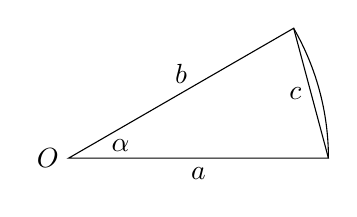
\begin{tikzpicture}[scale=1.1]
  \coordinate  (A) at (3,0);
  \coordinate[label = left:$O$] (O) at (0,0);
  \vertex{O};
  \draw (A) arc(0:30:3) coordinate (B);
  \draw (A) -- node[below] {$a$} (O) -- node[above] {$b$} (B) -- node[left] {$c$} cycle;
  \node[above right,xshift=12pt,yshift=-1pt] at (O) {$\alpha$};
\end{tikzpicture}
\caption{Die Länge einer Sehne, die einem Bogen der Größe $\alpha$}\label{fig.length-of-a-chord}
\end{center}
\end{figure}
\begin{eqnarray*}
c^2&=&a^2+b^2-2ab\cos \alpha\\
c&=&\sqrt{2-2\cos \alpha}\\
\lim_{\alpha\rightarrow 0} c&=& \sqrt{2-2\cdot 1}=0\,.
\end{eqnarray*}
Bezug nehmend auf Abb.~\ref{fig.ratio-of-sine-to-x}:
\[
\lim_{\alpha \rightarrow 0} \frac{\sin \alpha}{\alpha} = \lim_{\alpha \rightarrow 0} \frac{2\sin \alpha}{2\alpha}\,.
\]
Dies ist das Verhältnis zwischen der Länge der Sehne $\overline{PQ}$ und der Länge des Bogens $\widehat{PQ}$.
Wir haben aber gesehen, dass dieses Verhältnis gegen $1$ konvergiert, wenn der unterstellte Winkel $2\alpha$ gegen $0$ tendiert, also:
\[
\lim_{\alpha \rightarrow 0} \frac{\sin \alpha}{\alpha} = 1\,.
\]
\end{proof}


\begin{figure}[bt]
\begin{center}
\begin{tikzpicture}[scale=.9]
  \draw[thin] (-2,0) -- (2,0);
  \draw[thin] (0,-2) -- (0,2);
  \coordinate[label = above left:$A$]  (A) at (-2,0);
  \coordinate[label = above right:$B$] (B) at (2,0);
  \coordinate[label = above left:$O$] (O) at (0,0);
\vertex{O};
  \node[above right,xshift=6pt] at (O) {$\alpha$} 
    node[below right,xshift=6pt] {$\alpha$};
  \coordinate (P) at (40:2);
  \node[above right] at (P) {$P$};
  \coordinate (Q) at (-40:2);
  \node[draw, name path = circle] at (O)
    [circle through = (A)] {};
  \draw (B)
    arc[start angle=0,end angle=40,radius=2cm];
  \draw (B)
    arc[start angle=0,end angle=-40,radius=2cm];
  \node at (2.1,.8) {$\alpha$};
  \node at (2.1,-.8) {$\alpha$};
  \draw[<->] (P) -- node[fill=white,xshift=-4pt] {$\sin \alpha$}
    (P |- O) coordinate (D);
  \draw[<->] (D) -- node[fill=white,xshift=-4pt] {$\sin \alpha$} (Q);
  \node[below right] at (Q) {$Q$};
  \draw (Q) -- node[below] {$1$} (O) -- node[above] {$1$} (P);
\end{tikzpicture}
\caption{Verhältnis von $\sin x$ zu $x$}\label{fig.ratio-of-sine-to-x}
\end{center}
\end{figure}

%%%%%%%%%%%%%%%%%%%%%%%%%%%%%%%%%%%%%%%%%%%%%%%%%%%%%%%%%%%

\section{Der Satz von der Winkelhalbierenden}\label{a.bisector}


\begin{theorem}\label{thm.angle-bisector}
Im $\triangle ABC$ schneidet die Winkelhalbierende von $\angle BAC$ die $\overline{BC}$ in $D$ (Abb.~\ref{f.angle-bisector}). Dann:
\[
\frac {\overline{BD}}{\overline{CD}}=\frac {\overline{AB}}{\overline{AC}}\,.
\]
\end{theorem}

\begin{figure}[b]
\begin{center}
\begin{tikzpicture}[scale=.8]
% Draw base and path two lines at known angles
\draw (0,0) coordinate (b) node[left] {$B$} -- (8,0) coordinate (c) node[right] {$C$};
\path[name path=ba] (b) -- +(50:4.5);
\path[name path=ca] (c) -- +(150:7);
% Get their intersection and draw lines between vertices
\path[name intersections={of=ba and ca,by=a}];
\node[above] at (a) {$A$};
\draw (a) -- (c) -- (b) -- (a);
\path[name path=bc] (b) -- (c);
\path[name path=bisector] (a) -- +(-80:4);
\path[name intersections={of= bc and bisector,by=d}];
\node[below] at (d) {$D$};
\draw (a) -- (d);
\node[below left,xshift=2pt,yshift=-8pt] at (a) {$\alpha$};
\node[below right,xshift=2pt,yshift=-8pt] at (a) {$\alpha$};
\draw (a) -- node[left] {$h$} (a |- b);
\draw (a|-b) rectangle +(7pt,7pt);
\end{tikzpicture}
\end{center}
\caption{Der Satz von der inneren Winkelhalbierenden}\label{f.angle-bisector}
\end{figure}
\begin{proof}
Wir beweisen den Satz, indem wir die Flächen zweier Dreiecke berechnen, indem wir sowohl die Basis und die Höhe (Gl.~\ref{eq.area-from-base}), als auch die Basis, den Winkel und die Seite (Gl.~\ref{eq.area-from-sine}) verwenden:
\begin{eqnarray*}
\triangle ABD&=&\frac{1}{2}\overline{BD}h=\frac{1}{2}\overline{AB}\,\overline{AD}\sin \alpha\\
\frac{\overline{BD}}{\overline{AB}}&=&\frac{\overline{AD}\sin \alpha}{h}\\
\triangle ACD&=&\frac{1}{2}\overline{CD}h=\frac{1}{2}\overline{AC}\,\overline{AD}\sin \alpha\\
\frac{\overline{CD}}{\overline{AC}}&=&\frac{\overline{AD}\sin \alpha}{h}\\
\frac{\overline{BD}}{\overline{CD}}&=&\frac{\overline{AB}}{\overline{AC}}\,.
\end{eqnarray*}
\end{proof}
Es gibt auch einen Winkelhalbierungssatz für die \emph{externe Winkelhalbierung}:

\begin{theorem}\label{thm.external-angle-bisector}
Im $\triangle ABC$ sei $\overline{AE}$ die Winkelhalbierende des Winkels, der zum Winkel $\triangle BAC$ (Abb.~\ref{f.angle-bisector-external}) hinzukommt, und die Winkelhalbierende schneide $\overline{BC}$ in $E$ (Abb.~\ref{f.angle-bisector}). Dann:
\[
\frac {\overline{BE}}{\overline{CE}}=\frac {\overline{AB}}{\overline{AC}}\,.
\]
\end{theorem}

\begin{figure}[t]
\begin{center}
\begin{tikzpicture}[scale=1]
% Draw base and path two lines at known angles
\draw (0,0) coordinate (b) node[below] {$B$} -- (6,0) coordinate (c) node[right] {$C$};
\path[name path=ba] (b) -- +(70:2.5);
\draw[name path=ca] (c) -- +(160:7);
% Get their intersection and draw lines between vertices
\path[name intersections={of=ba and ca,by=a}];
\node[above] at (a) {$A$};
\draw (a) -- (c) -- (b) -- (a);
\path[name path=bc] (b) -- (c);
\node[left,xshift=-10pt,yshift=-2pt] at (a) {$\alpha$};
\node[below,xshift=-12pt,yshift=-8pt] at (a) {$\alpha$};
\path[name path=ext-bisector] (a) -- +(-155:4.7);
\draw[name path=ext-bc] (c) -- ($(c)!1.6!(b)$);
\path[name intersections={of=ext-bc and ext-bisector,by=e}];
\draw (a) -- (e) node[below] {$E$};
\coordinate (d) at (a |- b);
\draw (a) -- node[right] {$h$} (d);
\draw (d) rectangle +(6pt,6pt);
\end{tikzpicture}
\end{center}
\caption{Der Satz von der äußeren Winkelhalbierenden}\label{f.angle-bisector-external}
\end{figure}
\begin{proof} Da $\overline{AC}$ eine gerade Linie ist $\angle EAC=180^\circ-\alpha$.
\begin{eqnarray*}
\triangle ABE&=&\frac{1}{2}\overline{BE}h=\frac{1}{2}\overline{AE}\,\overline{AB}\sin \alpha\\
\triangle ACE&=&\frac{1}{2}\overline{CE}h=\frac{1}{2}\overline{AE}\,\overline{AC}\sin (180^\circ-\alpha)=\frac{1}{2}\overline{AE}\,\overline{AC}\sin \alpha\\
\frac{\overline{BE}}{\overline{AB}}&=&\frac{\overline{AE}\sin \alpha}{h}=\frac{\overline{CE}}{\overline{AC}}\\
\frac{\overline{BE}}{\overline{CE}}&=&\frac{\overline{AB}}{\overline{AC}}\,.
\end{eqnarray*}
\end{proof}

%%%%%%%%%%%%%%%%%%%%%%%%%%%%%%%%%%%%%%%%%%%%%%%%%%%%%%%%%%%

\section{Ptolemäus' Theorem}\label{a.ptolemy}


%%%%%%%%%%%%%%%%%%%%%%%%%%%%%%%%%%%%%%%%%%%%%%%%%%%%%%%%%%%

\subsection{Ein von einem Kreis umschriebenes Trapez}\label{s.circumscribed}

Vor dem Beweis des Satzes von Ptolemäus werden Theoreme über Vierecke und Trapeze bewiesen.

\begin{theorem}\label{thm.quad-circum}
Ein Viereck kann nur dann von einem Kreis umschrieben werden, wenn die gegenüberliegenden Winkel ergänzend sind (Summe $180^\circ$).
\end{theorem}

In den Geometrie-Lehrbüchern findet man den einfachen Beweis für die Vorwärtsrichtung, aber es ist schwierig, einen Beweis für die Umkehrung zu finden, so dass hier beide Beweise gegeben werden.

\begin{proof}(Vorwärtsrichtung)
Ein eingeschriebener Winkel ist gleich der Hälfte des Bogens, der ihn unterspannt, so dass $\angle DAB$ die Hälfte des Bogens $\widehat{DCB}$ ist und $\angle DCB$ die Hälfte des Bogens $\widehat{DAB}$ (Abb.~\ref{f.trap-1}). Die beiden Bögen bilden den gesamten Umfang des Kreises, so dass ihre Summe $360^\circ$ beträgt. Daher ist $\angle DAB + \angle DCB = \frac{1}{2} \cdot 360^\circ = 180^\circ$, und in ähnlicher Weise $\angle ADC + \angle ABC = 180^\circ$.
\end{proof}
\begin{figure}[tb]
\begin{minipage}{.45\textwidth}
\begin{tikzpicture}[scale=.55]
\coordinate (origin) at (0,0);
\coordinate (A) at (1,3);
\node[draw,circle through=(A),name path=circle] at (origin) {};
\node[above right] at (A) {$A$};
\path[name path=b] (A) -- (-50:4.5cm);
\path[name path=c] (A) -- (-120:4.5cm);
\path[name path=d] (A) -- (150:4.5cm);
\path [name intersections={of=circle and b,by={b1,B}}];
\node[right] at (B) {$B$};
\path [name intersections={of=circle and c,by={c1,C}}];
\node[below left] at (C) {$C$};
\path [name intersections={of=circle and d,by={d1,D}}];
\node[above left] at (D) {$D$};
\draw (A) -- (B) -- (C) -- (D) -- cycle;
\end{tikzpicture}
\caption{Ein Viereck, das von einem Kreis umschrieben wird}\label{f.trap-1}
\end{minipage}
\hfill
\begin{minipage}{.45\textwidth}
\begin{tikzpicture}[scale=.55]
\coordinate (origin) at (0,0);
\coordinate (A) at (1,3);
\node[draw,circle through=(A),name path=circle] at (origin) {};
\node[above right] at (A) {$A$};
\path[name path=b] (A) -- (-50:4cm);
\path[name path=c] (A) -- (-120:4cm);
\path[name path=d] (A) -- (150:4cm);
\path [name intersections={of=circle and b,by={b1,B}}];
\node[right] at (B) {$B$};
\path [name intersections={of=circle and c,by={c1,C}}];
\node[below left] at (C) {$C$};
\path [name intersections={of=circle and d,by={d2,D}}];
\node[above left] at (D) {$D$};
\coordinate (Cp) at ($(C)!.2!(D)$);
\draw (A) -- (B) -- (Cp) -- (D) -- cycle;
\node[left,xshift=1pt,yshift=2pt] at (Cp) {$C'$};
\draw (D) -- (B) -- (C) -- (Cp);
\end{tikzpicture}
\caption{Der vierte Scheitelpunkt muss auf dem Kreisumfang liegen}\label{f.trap-2}
\end{minipage}
\end{figure}

\begin{proof}(Umgekehrte Richtung)
Jedes Dreieck kann von einem Kreis umschrieben werden. Umschreibe das $\triangle DAB$ durch einen Kreis und nimm an, dass $C'$ ein solcher Punkt ist, dass $\angle DAB + \angle DC'B = 180^\circ$, aber $C'$ nicht auf dem Kreisumfang liegt. Ohne Verlust der Allgemeinheit sei $C'$ innerhalb des Kreises (Abb.~\ref{f.trap-2}).

Konstruieren Sie einen Strahl, der $\overline{DC'}$ verlängert, und lassen Sie $C$ seinen Schnittpunkt mit dem Kreis sein. $\overline{ABCD}$ wird also von einem Kreis umschrieben:
\begin{eqnarray*}
\angle DAB + \angle DCB &=&  180^\circ = \angle DAB + \angle DC'B\\
\angle DCB &=& \angle DC'B\,,
\end{eqnarray*}
was nicht möglich ist, wenn $C$ auf dem Kreis liegt und $C'$ innerhalb des Kreises liegt.
\end{proof}

\begin{theorem}\label{thm.isoceles-trapezoid}
Die gegenüberliegenden Winkel eines gleichschenkligen Trapezes sind ergänzend.
\end{theorem}
\begin{proof}
Konstruieren Sie die Linie $\overline{AB'}$ parallel zu $\overline{CD}$ (Abb.~\ref{f.trap-3}). $\overline{AB'CD}$ ist ein Parallelogramm und $\triangle ABB'$ ist ein gleichschenkliges Dreieck, also $\angle C= \angle ABB' = \angle AB'B = \angle B$. Ähnlich verhält es sich mit $\angle A = \angle D$. Da die Summe der Innenwinkel eines beliebigen Vierecks gleich $360^\circ$ ist:
\begin{eqnarray*}
\angle A + \angle B + \angle C + \angle D &=& 360^\circ\\
2\angle A + 2 \angle C &=& 360^\circ\\
\angle A +  \angle C &=& 180^\circ\,,
\end{eqnarray*}
und in ähnlicher Weise $\angle B +  \angle D = 180^\circ$.
\end{proof}
\begin{theorem}
Ein isozyklisches Trapez kann von einem Kreis umschrieben werden.
\end{theorem}
Der Beweis ist unmittelbar durch Thms.~\ref{thm.quad-circum}, \ref{thm.isoceles-trapezoid}.

\begin{figure}[t]
\begin{center}
\begin{tikzpicture}[scale=.65]
\clip (-4.5,-2) rectangle (4.5,2.8);
\coordinate (origin) at (0,0);
\coordinate (A) at (2.5,1.8);
\node[circle through=(A),name path=circle] at (origin) {};
\node[above right] at (A) {$A$};
\path[name path=b] (A) -- ++(-80:4cm);
\path[name path=d] (A) -- ++(180:6cm);
\path [name intersections={of=circle and b,by={b1,B}}];
\node[below right] at (B) {$B$};
\path [name intersections={of=circle and d,by={d1,D}}];
\node[above left] at (D) {$D$};
\path[name path=c] (D) -- ++(-100:4cm);
\path [name intersections={of=circle and c,by={c1,C}}];
\node[below left] at (C) {$C$};
\draw (A) -- node[right] {$x$} (B);
\draw[name path=bc] (B) -- node[below] {$y$} (C);
\draw (C) -- node[left] {$x$} (D) -- node[above] {$y$} (A);
\path[name path=para] (A) -- ++(-100:4cm);
\path [name intersections={of=para and bc,by={Bp}}];
\node[below left] at (Bp) {$B'$};
\draw (A) -- node[left,xshift=-2pt] {$x$} (Bp);
\end{tikzpicture}
\end{center}
\caption{Ein isoceles Trapez}\label{f.trap-3}
\end{figure}

%%%%%%%%%%%%%%%%%%%%%%%%%%%%%%%%%%%%%%%%%%%%%%%%%%%%%%%%%%%

\subsection{Beweis des Satzes von Ptolemäus}

\begin{theorem}(Ptolemy)
Bei einem Viereck, das von einem Kreis umschrieben wird, setzt die folgende Formel die Längen der Diagonalen und der Seiten in Beziehung (Abb.~\ref{f.trig-ptolemy}).\label{thm.ptolemy}
\[
ef = ac + bd\,.
\]
\end{theorem}

\begin{figure}[b]
\begin{center}
\begin{tikzpicture}[scale=.5]
\coordinate (origin) at (0,0);
\coordinate (A) at (1,3);
\node[draw,circle through=(A),name path=circle] at (origin) {};
\node[above right] at (A) {$A$};
\path[name path=b] (A) -- (-50:4cm);
\path[name path=c] (A) -- (-120:4cm);
\path[name path=d] (A) -- (150:4cm);
\path [name intersections={of=circle and b,by={b1,B}}];
\node[right] at (B) {$B$};
\path [name intersections={of=circle and c,by={C,c2}}];
\node[below left] at (C) {$C$};
\path [name intersections={of=circle and d,by={D,d2}}];
\node[above left] at (D) {$D$};
\draw (A) -- node[right] {$a$} (B) -- node[below,yshift=-10pt] {$b$} (C) -- node[left] {$c$} (D) -- node[above,xshift=2pt,yshift=8pt] {$d$}  cycle;
\draw (A) -- node[right,near start] {$e$} (C);
\draw (B) -- node[left,near end,yshift=-6pt] {$f$} (D);
\end{tikzpicture}
\end{center}
\caption{Ptolemäus' Theorem}\label{f.trig-ptolemy}
\end{figure}                       

\begin{proof}
Nach dem Kosinusgesetz für die vier Dreiecke $\triangle ABC$, $\triangle ADC$, $\triangle DAB$, $\triangle DCB$:
\begin{eqnarray*}
e^2 &=& a^2 + b^2 - 2ab \cos \angle B\\
e^2 &=& c^2 + d^2 - 2cd \cos \angle D\\
f^2 &=& a^2 + d^2 - 2ad \cos \angle A\\
f^2 &=& b^2 + c^2 - 2bc \cos \angle C\,.
\end{eqnarray*}
$\angle C = 180^\circ - \angle A$ und $\angle D = 180^\circ - \angle B$, weil sie entgegengesetzte Winkel eines von einem Kreis umschriebenen Vierecks sind, also $\cos \angle D = - \cos \angle B$ und $\cos \angle C = -\cos \angle A$. Eliminiert man den Kosinusterm aus den obigen Gleichungen, erhält man:
\begin{eqnarray*}
e^2(cd+ab)&=&abc^2+abd^2+a^2cd+b^2cd\\
e^2 &=& \frac{(ac+bd)(ad+bc)}{(ab+cd)}\\
f^2 &=& \frac{(ab+cd)(ac+bd)}{(ad+bc)}\,.
\end{eqnarray*}
Multiplizieren Sie die beiden Gleichungen und vereinfachen Sie sie, um das Theorem von Ptolemäus zu erhalten:
\begin{eqnarray*}
e^2\cdot f^2 &=& (ac+bd)^2\\
ef &=& (ac+bd)\,.
\end{eqnarray*}
\end{proof}

%%%%%%%%%%%%%%%%%%%%%%%%%%%%%%%%%%%%%%%%%%%%%%%%%%%%%%%%%%%

\section{Cevas Theorem}\label{a.ceva}


\begin{theorem}(Ceva)
Bei Liniensegmenten von den Eckpunkten eines Dreiecks zu den gegenüberliegenden Kanten, die sich in einem Punkt schneiden, erfüllen die Längen der Segmente (Fig.~\ref{f.ceva1}):\label{thm.ceva}
\[
\frac{\overline{AM}}{\overline{MB}}\cdot\frac{\overline{BQ}}{\overline{QS}}\cdot\frac{\overline{SP}}{\overline{PA}} = 1\,.
\]
\end{theorem}

\begin{figure}[b]
\begin{center}
\begin{tikzpicture}
\path[name path=pq] (-4,0) -- (4,0);
\draw (-2,-2) node[below left] {$A$} coordinate (A) -- (2,-2) node[below right] {$B$} coordinate (B);
\draw[name path=as] (A) -- ++(50:4cm) node[above] {$S$} coordinate (S);
\draw[name path=sb] (S) -- (B);
\path [name intersections={of=pq and as,by={P}}];
\path [name intersections={of=pq and sb,by={Q}}];
\node[above left] at (P) {$P$};
\node[above right] at (Q) {$Q$};
\draw[name path=pb] (P) -- (B);
\draw[name path=qa] (Q) -- (A);
\path [name intersections={of=pb and qa,by={O}}];
\node[right,xshift=2pt] at (O) {$O$};
\coordinate (M) at (0,-2);
\node[below right] at (M) {$M$};
\draw (S) -- (M);
\end{tikzpicture}
\end{center}
\caption{Cevas Theorem}\label{f.ceva1}
\end{figure}

\begin{proof} Wenn die Höhen von zwei Dreiecken gleich sind, sind ihre Flächen proportional zu den Basen. In beiden Diagrammen in Abb.~\ref{f.ceva2} sind die Höhen der grauen Dreiecke gleich, also:
\[
\frac{\triangle BQO}{\triangle SQO} = \frac{\overline{BQ}}{\overline{QS}}\;,\quad\quad \frac{\triangle BQA}{\triangle SQA} = \frac{\overline{BQ}}{\overline{QS}}\;.
\]
Durch Subtraktion der Flächen der angegebenen Dreiecke erhält man das Verhältnis zwischen den grauen Dreiecken in Abb.~\ref{f.ceva3}:
\[
\frac{\triangle BOA}{\triangle SOA}=\frac{\triangle BQA - \triangle BQO}{\triangle SQA-\triangle SQO} = \frac{\overline{BQ}}{\overline{QS}}\,.
\]

\begin{figure}[t]
\begin{center}
\begin{tikzpicture}
\clip (-2.2,-2.4) rectangle +(10.4,4);
\path[name path=pq] (-4,0) -- (4,0);
\draw (-2,-2) node[below] {$A$} coordinate (A) -- (2,-2) node[below] {$B$} coordinate (B);
\coordinate (M) at (0,-2);
\draw[name path=as] (A) -- ++(50:4cm) node[above] {$S$} coordinate (S);
\draw[name path=sb] (S) -- (B);
\path [name intersections={of=pq and as,by={P}}];
\path [name intersections={of=pq and sb,by={Q}}];
\path[name path=pb] (P) -- (B);
\path[name path=qa] (Q) -- (A);
\path [name intersections={of=pb and qa,by={O}}];
\draw[fill=gray!40] (B) -- (O) -- (Q);
\draw[fill=gray!70] (S) -- (O) -- (Q);
\draw (B) -- (O) -- (A);
\draw (S) -- (O) -- (A);
\draw (A) -- (B) -- (S) -- cycle;
\draw (S) -- (O);
\draw (B) -- (O);
\node[above right] at (Q) {$Q$};
\node[above left] at (O) {$O$};
\path[name path=al1] (O) -- ($(Q)!(O)!(B)$);
\path [name intersections={of=al1 and sb,by={A1}}];
\draw (O) -- (A1);
\draw[rotate=-156] (A1) rectangle +(7pt,7pt);
\begin{scope}[xshift=6cm]
\path[name path=pq] (-4,0) -- (4,0);
\draw (-2,-2) node[below] {$A$} coordinate (A) -- (2,-2) node[below] {$B$} coordinate (B);
\coordinate (M) at (0,-2);
\draw[name path=as] (A) -- ++(50:4cm) node[above] {$S$} coordinate (S);
\draw[name path=sb] (S) -- (B);
\path [name intersections={of=pq and as,by={P}}];
\path [name intersections={of=pq and sb,by={Q}}];
\draw[name path=pb] (P) -- (B);
\draw[name path=qa] (Q) -- (A);
\path [name intersections={of=pb and qa,by={O}}];
\draw (B) -- (O) -- (Q);
\draw (A) -- (Q) -- (B);
\draw[fill=gray!40] (B) -- (Q) -- (A);
\draw[fill=gray!70] (S) -- (Q) -- (A);
\draw (A) -- (B) -- (S) -- cycle;
\draw (S) -- (O);
\draw (B) -- (O);
\node[above right] at (Q) {$Q$};
\node[above left] at (O) {$O$};
\path[name path=al2] (A) -- ($(Q)!(A)!(B)$);
\path [name intersections={of=al2 and sb,by={A2}}];
\draw (A) -- (A2);
\draw[rotate=-156] (A2) rectangle +(7pt,7pt);
\end{scope}
\end{tikzpicture}
\end{center}
\caption{Dreiecke in Cevas Theorem}\label{f.ceva2}
\end{figure}

\begin{figure}[b]
\begin{center}
\begin{tikzpicture}
\path[name path=pq] (-4,0) -- (4,0);
\draw (-2,-2) node[below left] {$A$} coordinate (A) -- (2,-2) node[below right] {$B$} coordinate (B);
\coordinate (M) at (0,-2);
\draw[name path=as] (A) -- ++(50:4cm) node[above] {$S$} coordinate (S);
\draw[name path=sb] (S) -- (B);
\path [name intersections={of=pq and as,by={P}}];
\path [name intersections={of=pq and sb,by={Q}}];
\path[name path=pb] (P) -- (B);
\draw[thick,name path=qa] (Q) -- (A);
\path [name intersections={of=pb and qa,by={O}}];
\draw[fill=gray!50] (B) -- (O) -- (A);
\draw[fill=gray!70] (S) -- (O) -- (A);
\draw (B) -- (O) -- (A);
\draw (S) -- (O) -- (A);
\draw (A) -- (B) -- (S) -- cycle;
\draw (S) -- (O);
\draw (B) -- (O);
\node[above right] at (Q) {$Q$};
\node[right,xshift=2pt] at (O) {$O$};
\end{tikzpicture}
\end{center}
\caption{Subtraktion von Flächen im Ceva-Theorem}\label{f.ceva3}
\end{figure}
Das mag auf den ersten Blick seltsam erscheinen, deshalb erklären wir es mit einer einfacheren Notation:
\begin{eqnarray*}
 \frac{c}{d} &=&\frac{a}{b}\\
 \frac{e}{f} &=&\frac{a}{b}\\
c-e &=& \frac{ad}{b} - \frac{af}{b}=\frac{a}{b}(d-f)\\
\frac{c-e}{d-f} &=& \frac{a}{b}\,.
\end{eqnarray*}
In ähnlicher Weise können wir beweisen:
\begin{eqnarray*}
\frac{\overline{AM}}{\overline{MB}} &=& \frac{\triangle AOS}{\triangle BOS}\\
\frac{\overline{SP}}{\overline{PA}} &=&\frac{\triangle SOB}{\triangle AOB}\;,
\end{eqnarray*}
so:
\[
\frac{\overline{AM}}{\overline{MB}}\frac{\overline{BQ}}{\overline{QS}}\frac{\overline{SP}}{\overline{PA}} = \frac{\triangle AOS}{\triangle BOS}\frac{\triangle BOA}{\triangle SOA}\frac{\triangle SOB}{\triangle AOB}=1\,,
\]
da die Reihenfolge der Scheitelpunkte in einem Dreieck keinen Unterschied macht.
\end{proof}

\begin{figure}[b]
\begin{center}
\begin{tikzpicture}[scale=.6]
\clip (-.8,-.4) rectangle +(11.2,6.5);
\coordinate (D) at (0,0) node[left] {$D$};
\draw (D) -- ++(60:6) coordinate (C) node[left] {$C$};
\coordinate (A) at (60:3);
\node[left] at (A) {$A$};
\draw (A) -- ++(3,0) coordinate (B) -- (C);
\node[below right] at (B) {$B$};
\path[name path=DQ] (D) -- ($(D)!1.7!(B)$);
\path[name path=AP] (A) -- ($(A)!3!(B)$);
% 3*(1+\sqrt[3]{2}) = 6.78
\path[name path=CP] (C) circle (6.78cm);
\path[name intersections={of=CP and AP,by={P}}];
\draw[name path=CP] (C) -- (P);
\path[name intersections={of=CP and DQ,by={Q}}];
\node[above] at (Q) {$Q$};
\node[right] at (P) {$P$};
\draw (D) -- (Q);
\draw (B) -- (P);
\path[dashed,name path=CK] (C) -- ($(C)+(6.5,0)$);
\path[name path=DK] (D) -- ($(D)!2!(Q)$);
\path[name intersections={of=DK and CK,by={K}}];
\draw[dashed] (Q) -- (K) node[right] {$K$} -- (C);
\draw[very thick] (Q) -- (D);
\draw[dashed] (C) -- (K) -- (Q);
\draw (B) -- (P) -- (C);
\end{tikzpicture}
\end{center}
\caption{Menelaos' Theorem}\label{f.menelaus}
\end{figure}

\section{Der Satz des Menelaos}\label{a.menelaus}

\begin{theorem}(Menelaos)\label{thm.menelaus}
Sei $\triangle ABC$ ein Dreieck und $\overline{DBQ}$ eine \emph{Transversallinie}, die alle drei Kanten des Dreiecks oder deren Erweiterungen schneidet (Abb.~\ref{f.menelaus}). Dann:\footnote{Abhängig von der Konfiguration des Dreiecks und der transversalen Linie kann das Ergebnis der Multiplikation entweder plus oder minus eins sein.}
\begin{align}
\displaystyle\frac{\overline{AB}}{\overline{BP}}\cdot
\displaystyle\frac{\overline{PQ}}{\overline{QC}}\cdot
\displaystyle\frac{\overline{CD}}{\overline{AD}}=1\,.\label{eq.menelaus}
\end{align}
\end{theorem}

\begin{proof}
Ziehe eine Linie durch $C$ parallel zu $\overline{AB}$ und verlängere $\overline{DQ}$, bis sie die Parallele in $K$ schneidet. Aus $\triangle ADB \sim \triangle CDK$ ergibt sich, dass:
\begin{equation*}
\displaystyle\frac{\overline{CD}}{\overline{AD}}=\displaystyle\frac{\overline{CK}}{\overline{AB}}\,.
\end{equation*}
Aus $\triangle BQP\sim \triangle KQC$ ergibt sich, dass:
\begin{equation*}
\displaystyle\frac{\overline{QC}}{\overline{PQ}}=\displaystyle\frac{\overline{CK}}{\overline{BP}}\,.
\end{equation*}
Die Eliminierung von $\overline{CK}$ ergibt
$\overline{AB}\cdot\overline{CD}\cdot\overline{PQ}=\overline{QC}\cdot\overline{BP}\cdot\overline{AD}$, das umgeordnet werden kann, um Gl.~\ref{eq.menelaus} zu erhalten.
\end{proof}

%%%%%%%%%%%%%%%%%%%%%%%%%%%%%%%%%%%%%%%%%%%%%%%%%%%%%%%%%%%

\subsection*{Quellen}

Der Anhang basiert in erster Linie auf \cite{gelfand}. Cevas Theorem und Menelaus' Theorem können aus einander bewiesen werden \cite{silvester}.
